%!TEX root=../../main.tex


\subsection{Single-source Shortest-paths}
For the results of our SSSP runs, we first analyze the single-node and distributed performances separately before comparing the two.

\subsubsection{Single-node}
Beginning with the single-node performance, \autoref{fig:singleNodeSSSP} shows the average calculation and execution times for SSSP on the different frameworks.

Because we did not see the perfomance going down when increasing thread counts on Galois, we always refer to Galois with 96 threads in this section (including the figures). 
For a more detailed analysis of Galois' behaviour with different thread counts, see \autoref{sec:galois_speedup}. 




TODO // Hier fehlt noch Giraph, daher noch keine vollständige Auswertung.
\begin{figure}
	\begin{subfigure}{0.3\textwidth}
		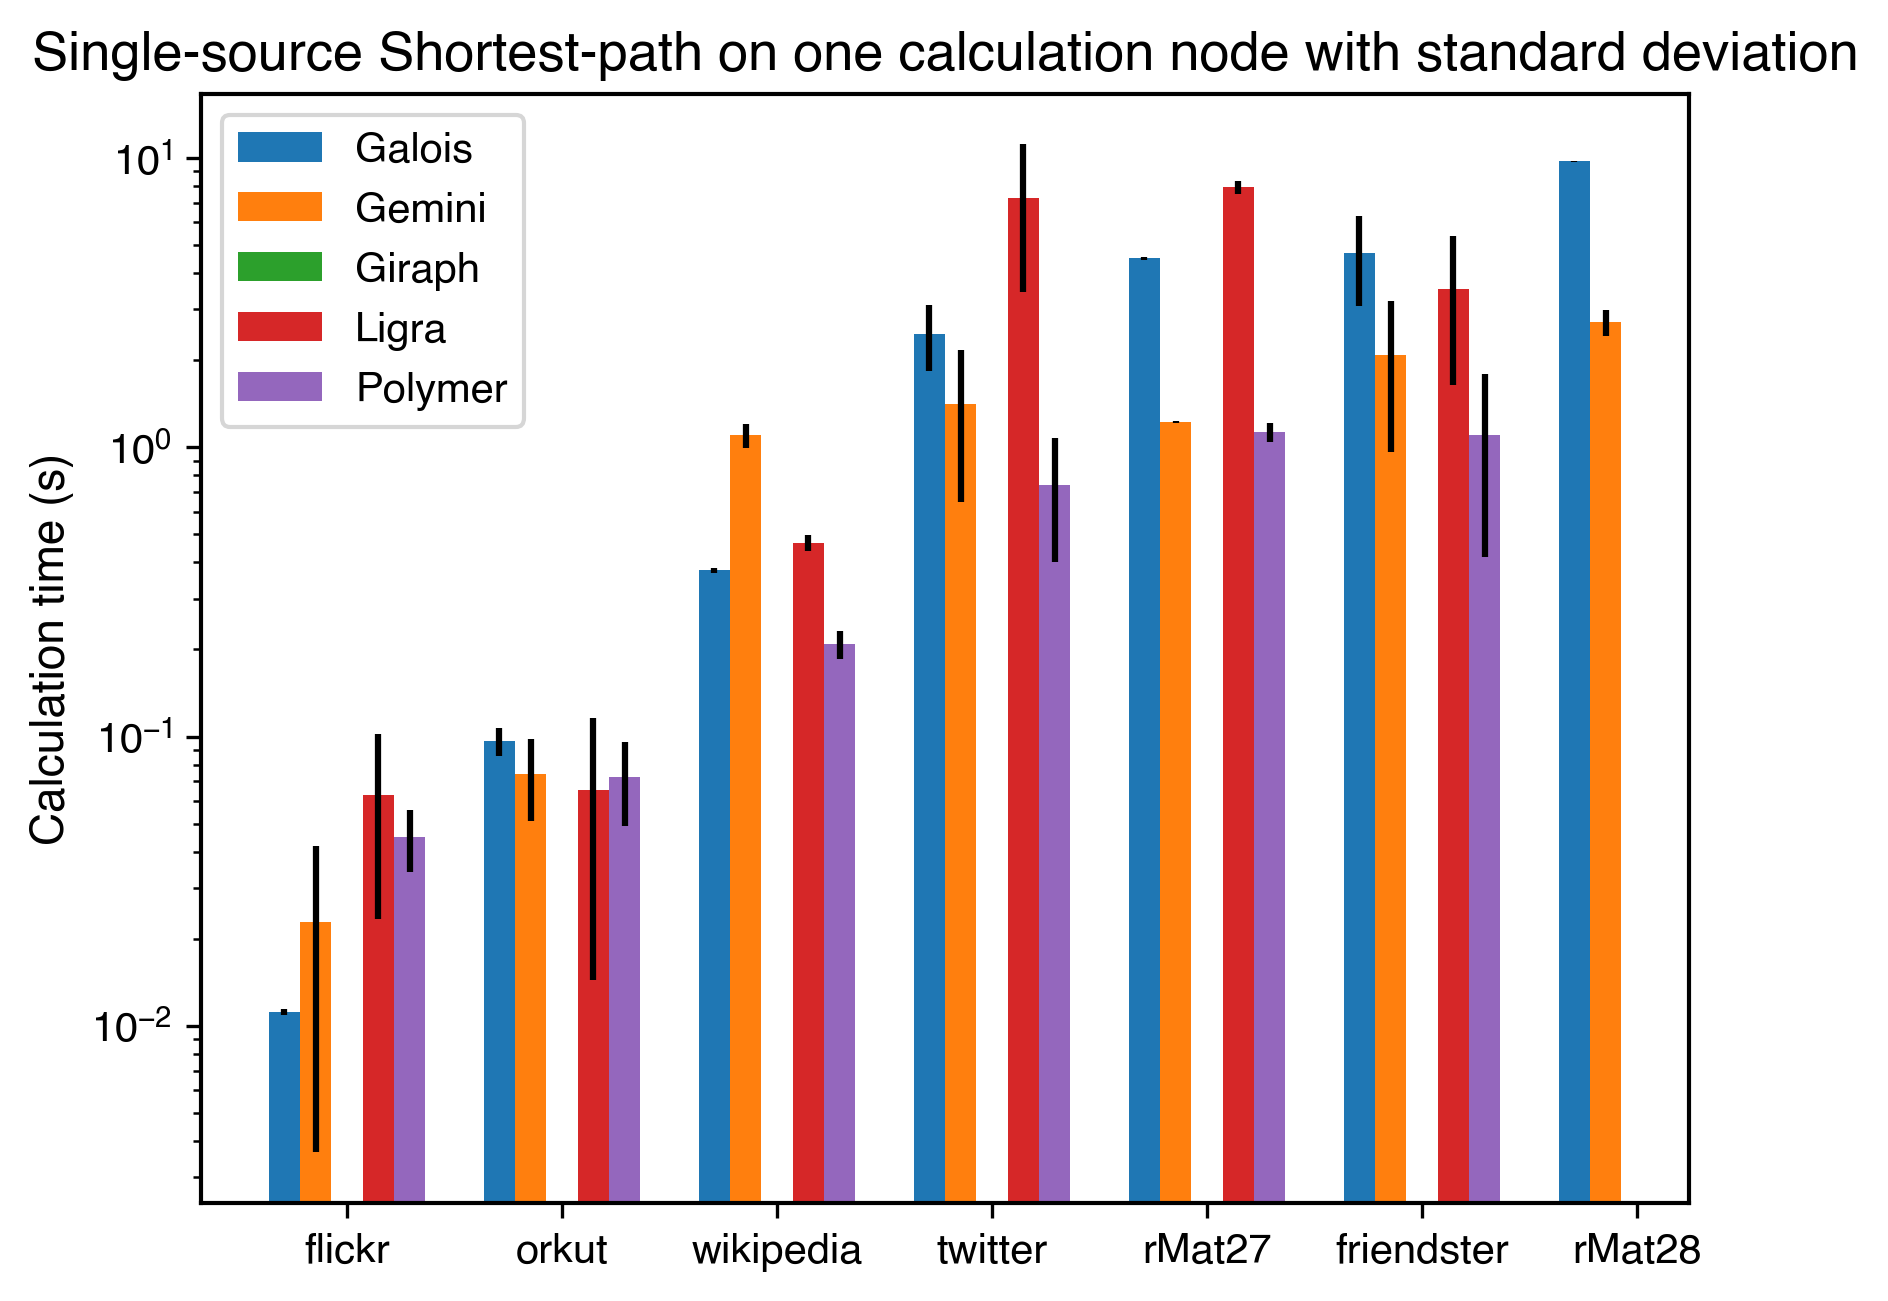
\includegraphics[width=\linewidth]{../../plots/singleNodeSSSP_calcTime.png}
		\caption{Calculation times for SSSP on a single node}
		\label{fig:singleNodeSSSP_calc}
	\end{subfigure}
	\hfil
	\begin{subfigure}{0.3\textwidth}
		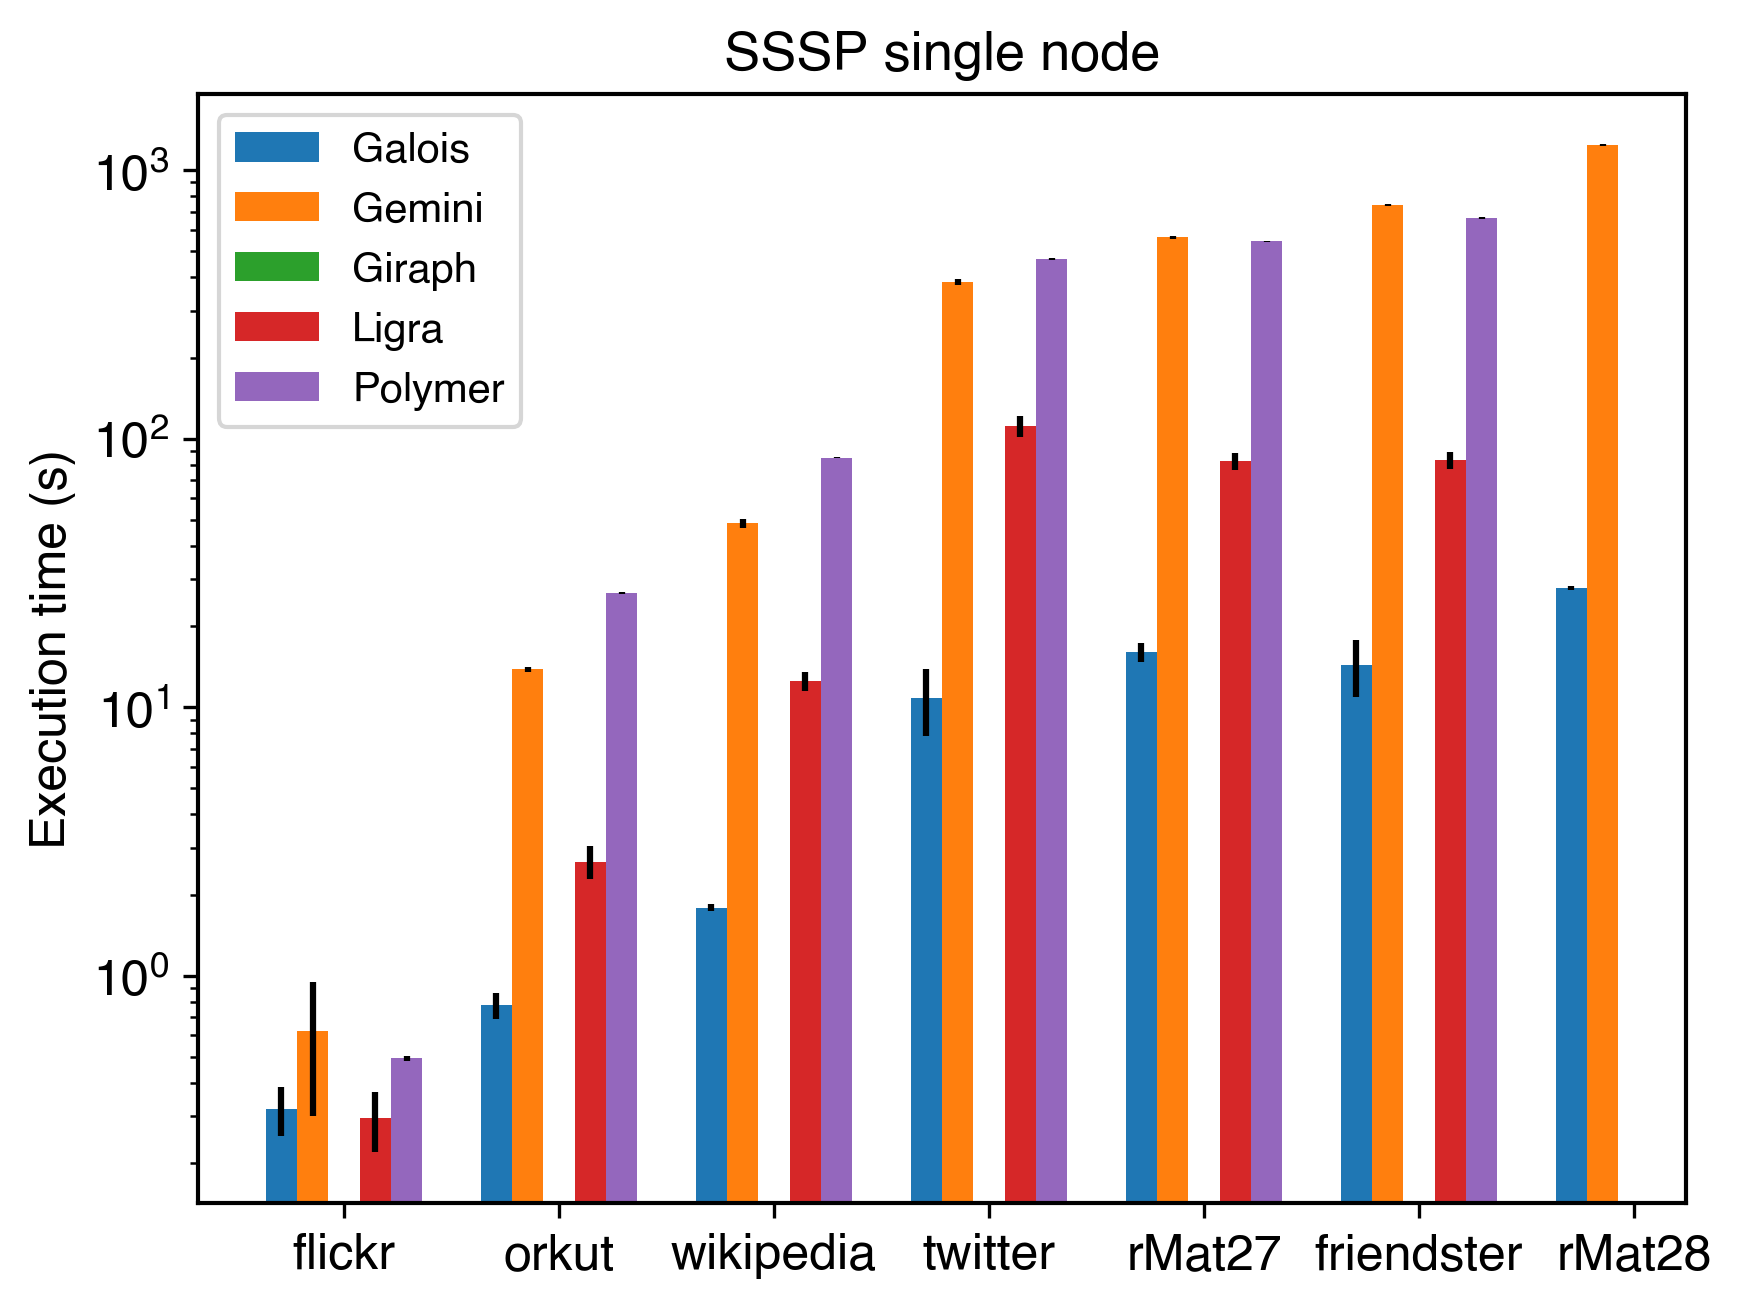
\includegraphics[width=\linewidth]{../../plots/singleNodeSSSP_execTime.png}
		\caption{Execution times for SSSP on a single node}
		\label{fig:singleNodeSSSP_exec}
	\end{subfigure}
	\hfil
	\begin{subfigure}{0.3\textwidth}
		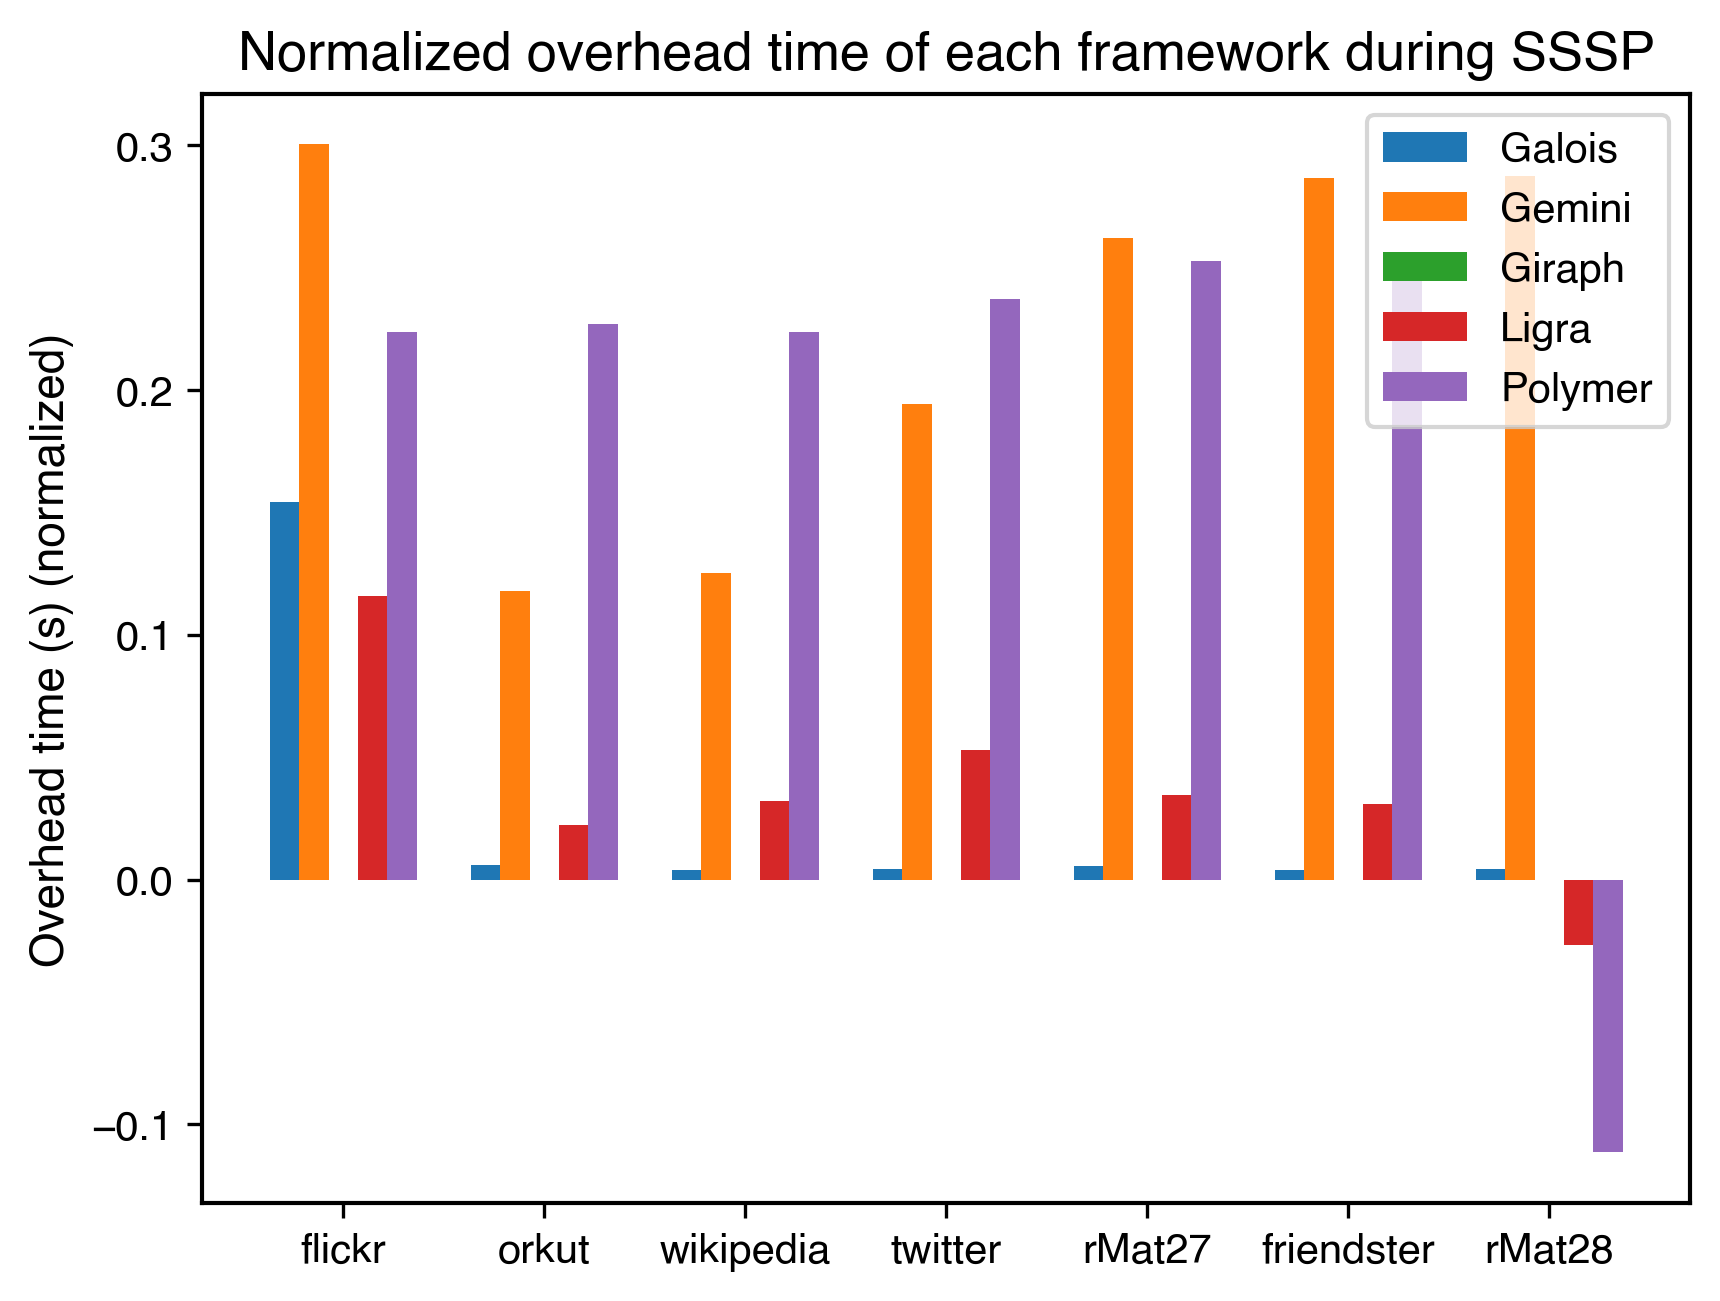
\includegraphics[width=\linewidth]{../../plots/singleNodeSSSP_overheadTimeNormalized.png}
		\caption{Overhead time normalized by the graph size in million edges}
		\label{fig:singleNodeSSSP_overheadNormalized}
	\end{subfigure}
	\caption{Average times on a single computation node, black bars represent one standard deviation in our testing.
	The runs on rMat28 for Ligra and Polymer failed and the frameworks were unable to complete the task.}
	\label{fig:singleNodeSSSP}
\end{figure}








\subsubsection{Distributed}

\begin{figure}
	\centering
	\begin{subfigure}{\columnwidth}
		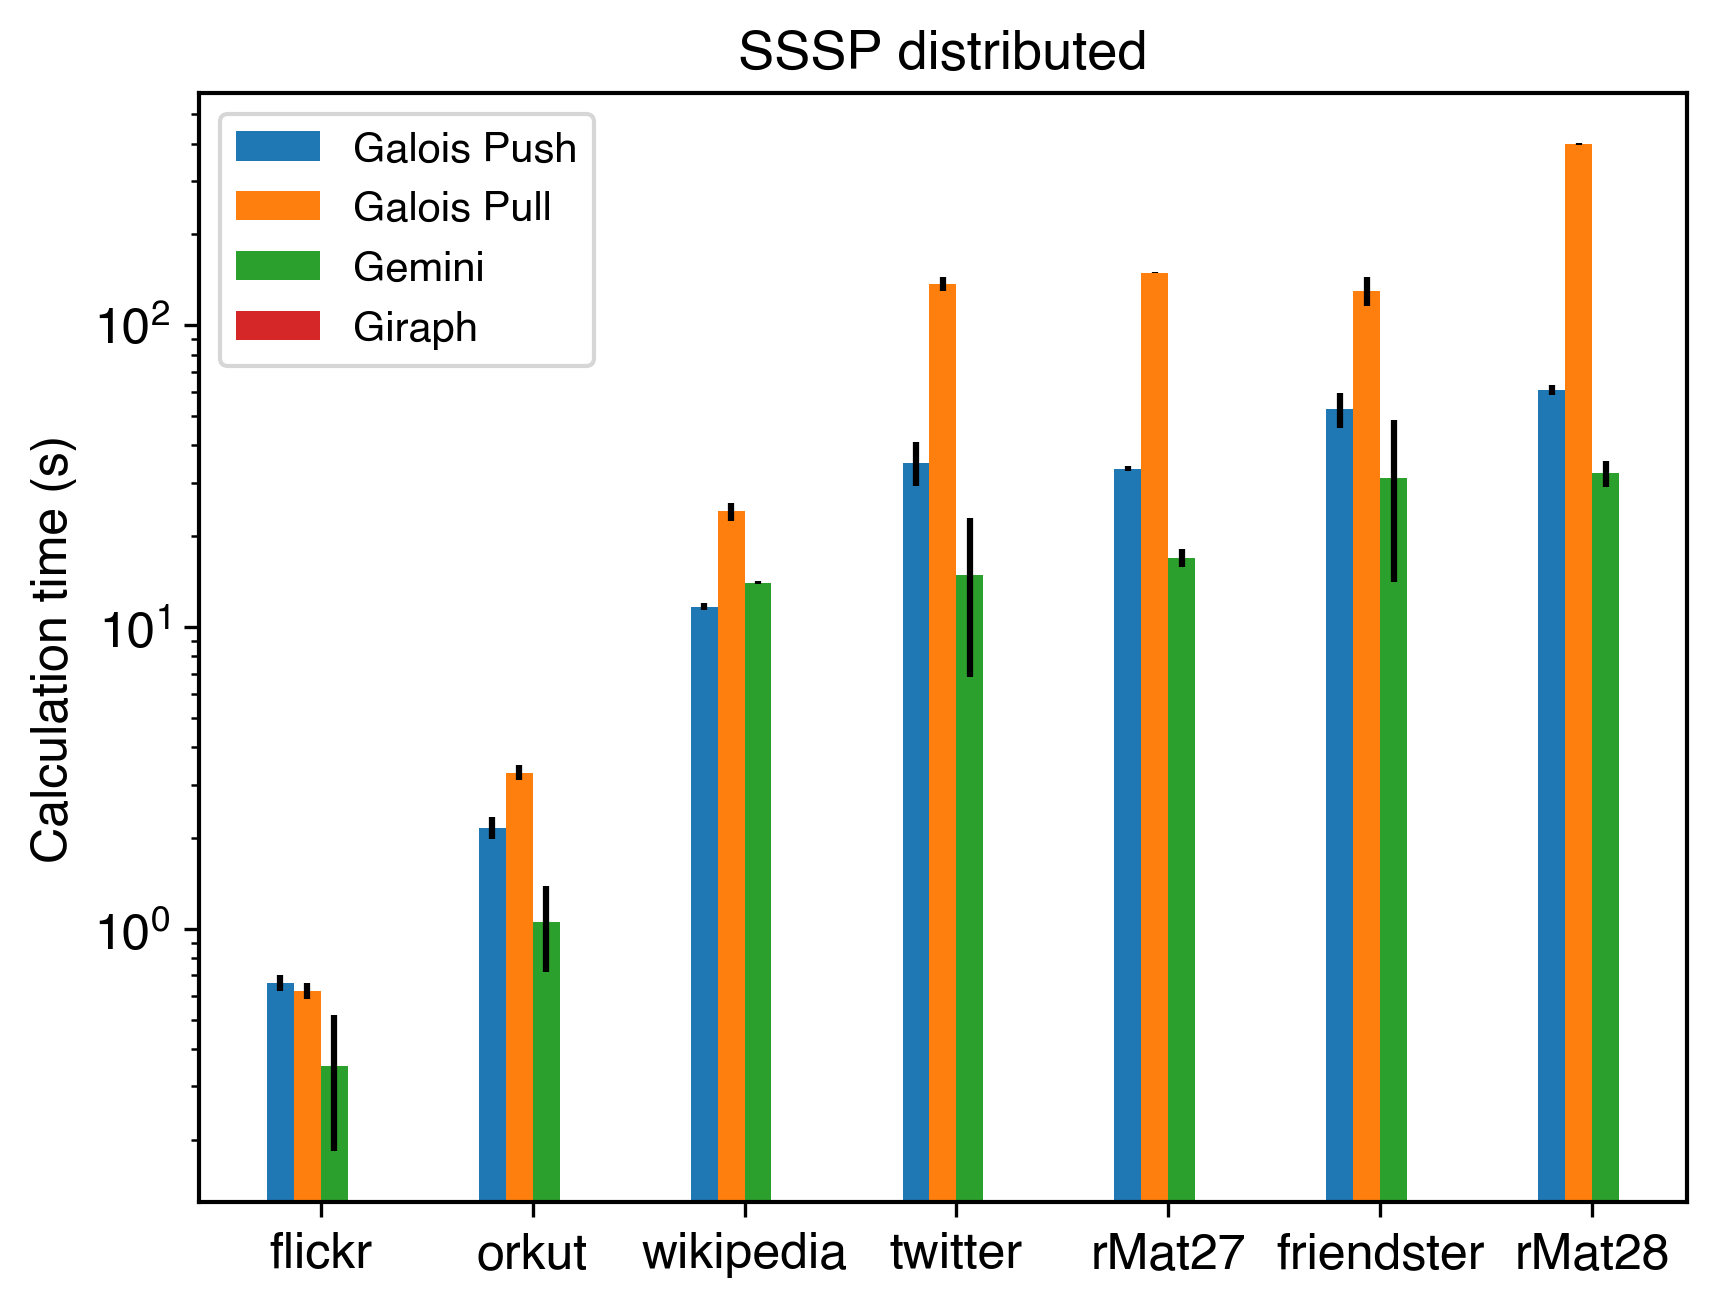
\includegraphics[width=\linewidth]{../../plots/distributedSSSP_calcTime.png}
		\caption{Calculation times for distributed SSSP}
		\label{fig:distributedSSSP_calc}
	\end{subfigure}
	\begin{subfigure}{\columnwidth}
		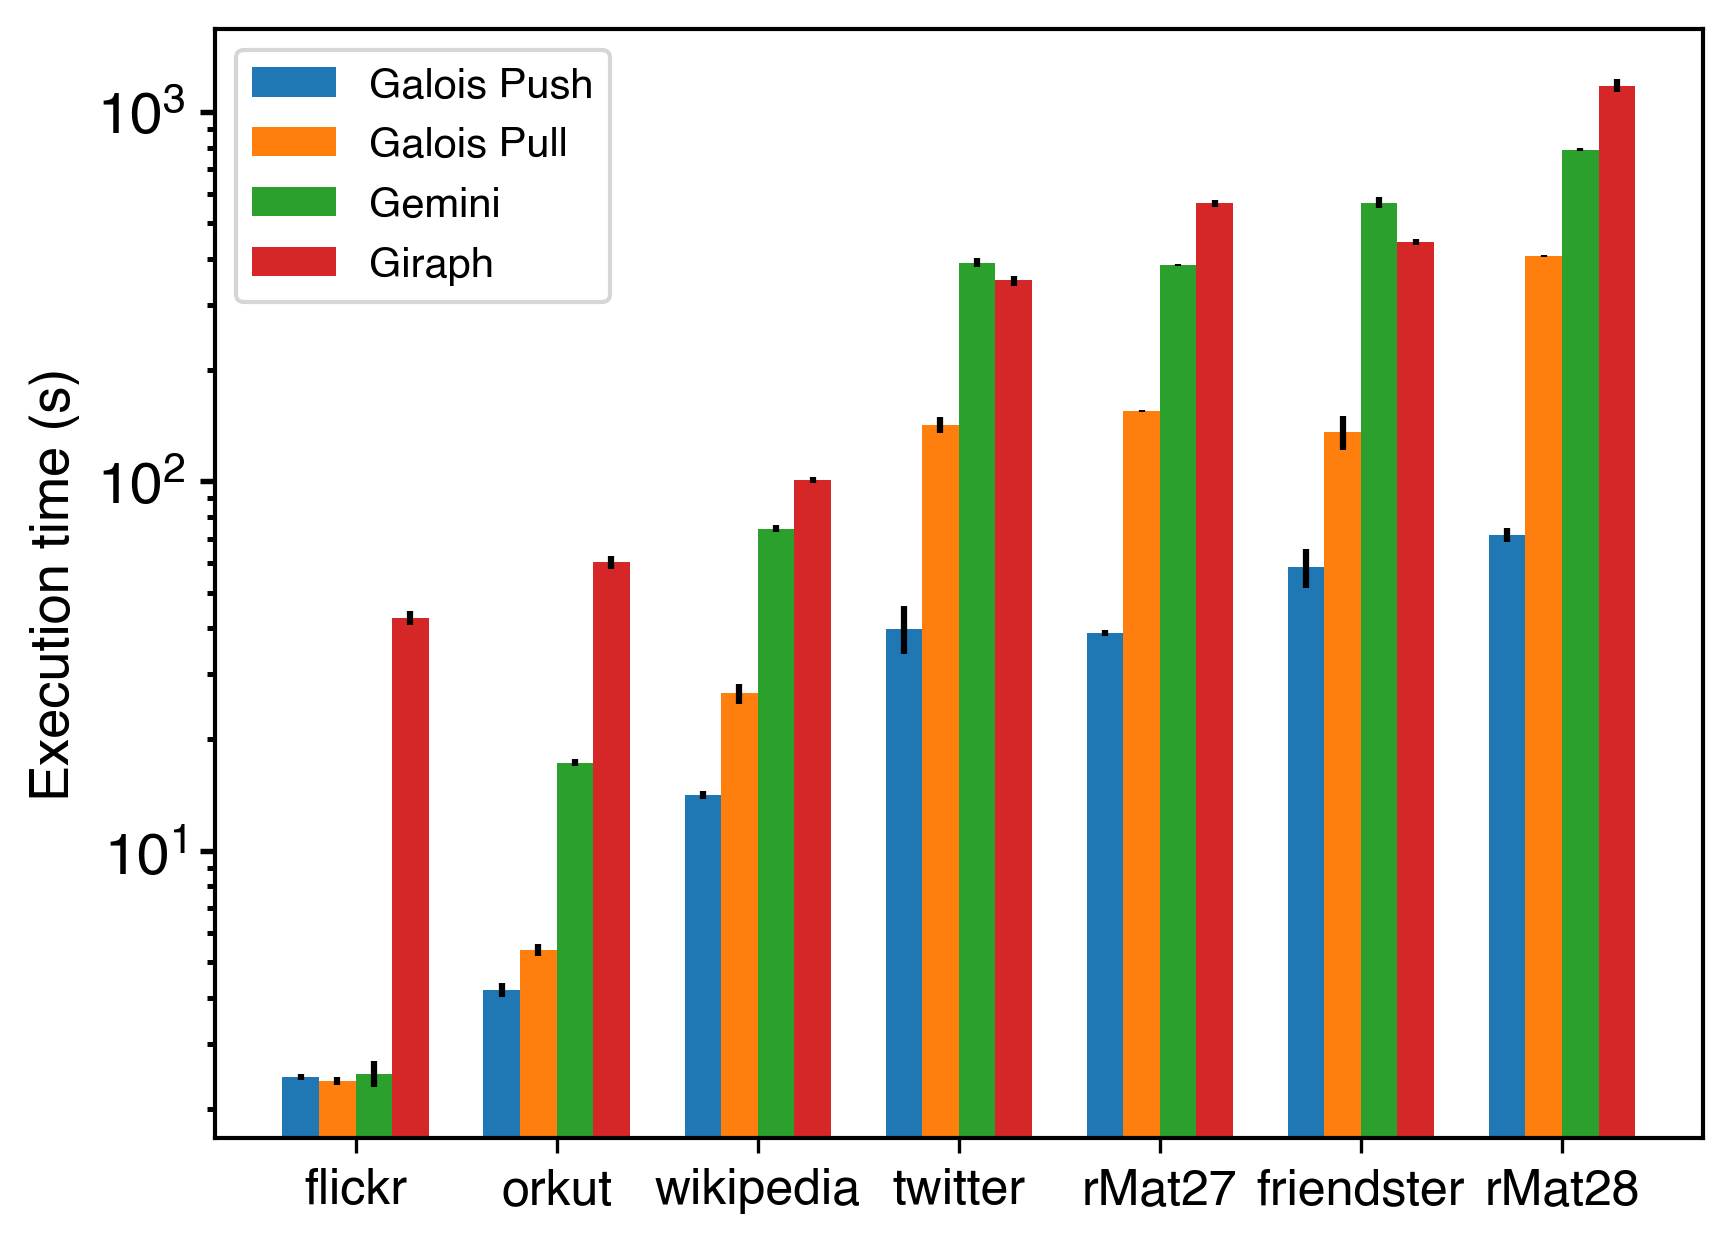
\includegraphics[width=\linewidth]{../../plots/distributedSSSP_execTime.png}
		\caption{Execution times for distributed SSSP}
		\label{fig:distributedSSSP_exec}
	\end{subfigure}
	\caption{Average times on the distributed cluster, black bars represent one standard deviation in our testing.}
	\label{fig:distributedSSSP}
\end{figure}

\begin{figure}
	\centering
	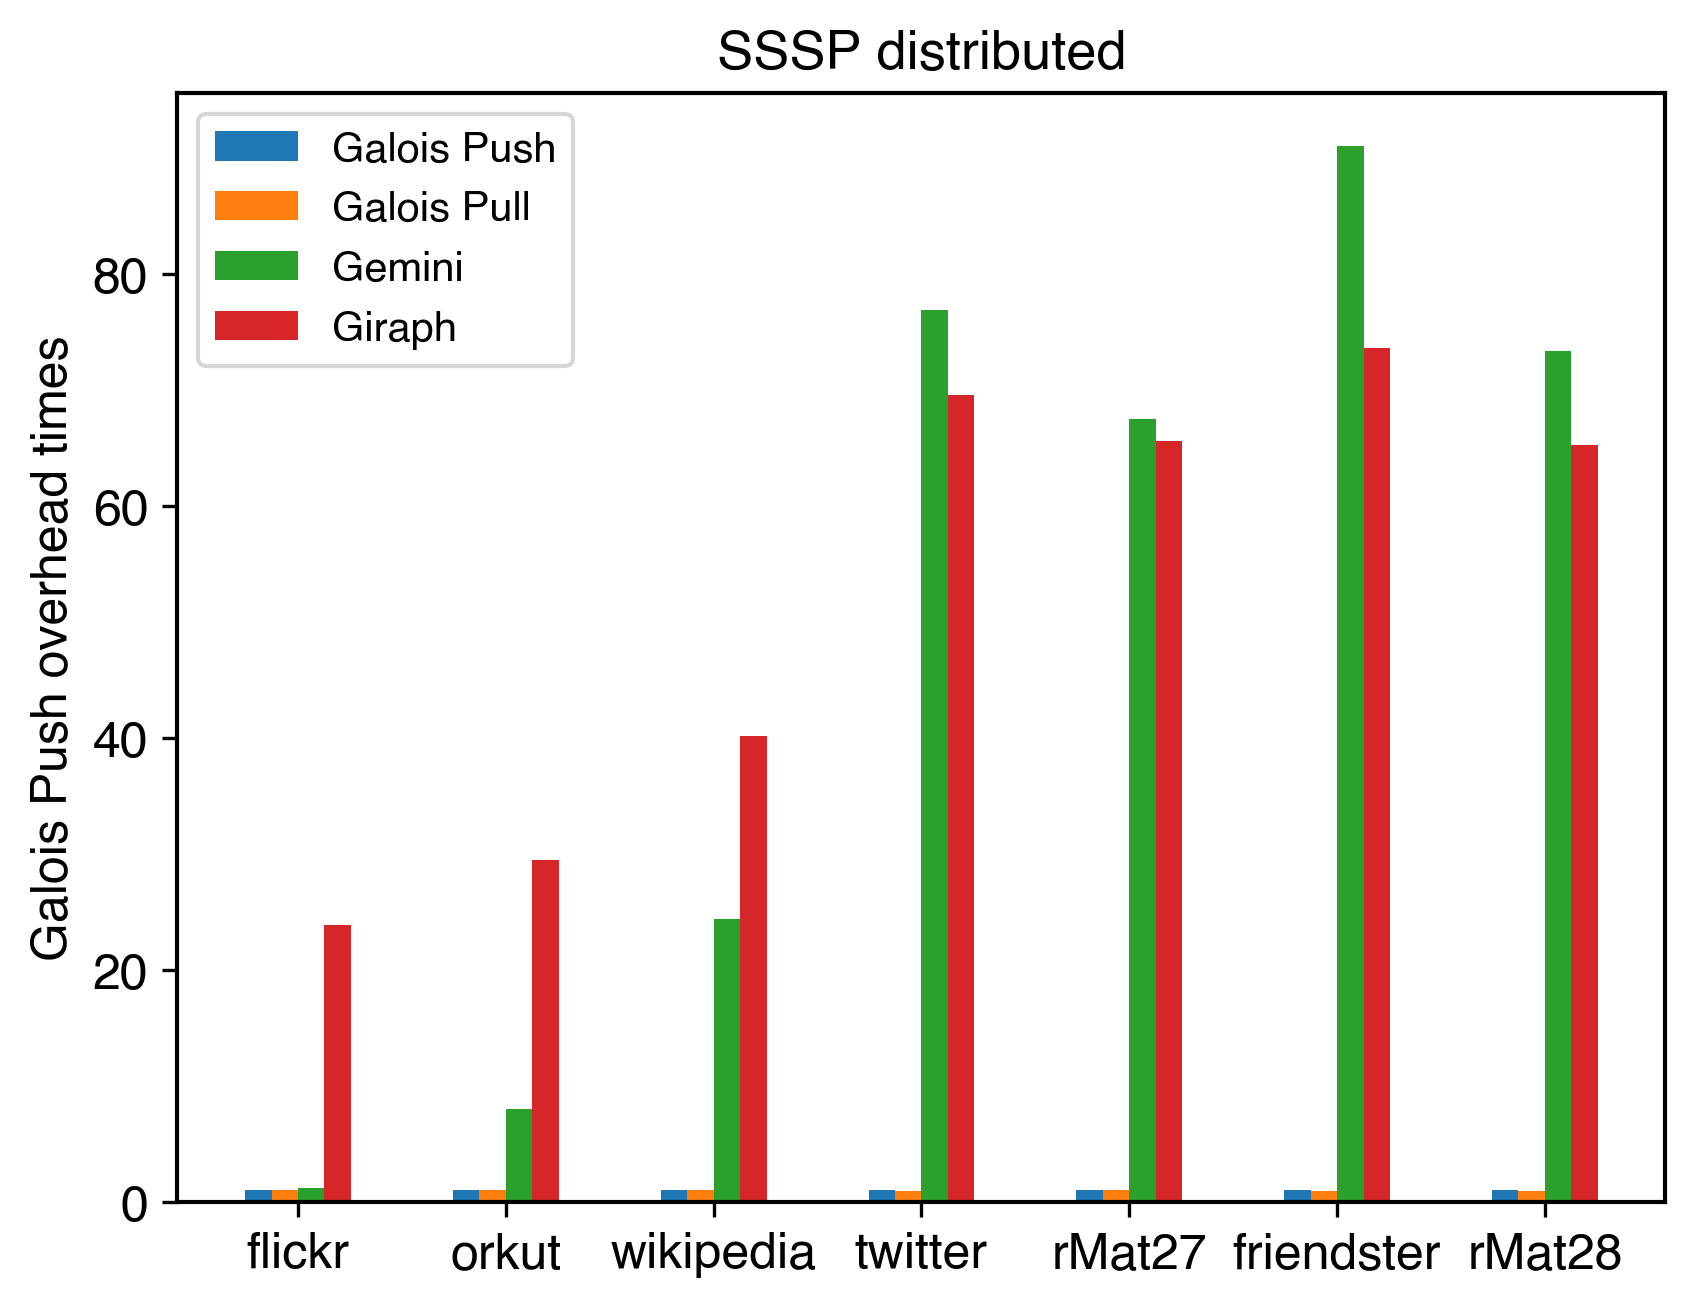
\includegraphics[width=\linewidth]{../../plots/distributedSSSP_overheadTimeNormalizedToGalois.png}
	\caption{Overhead times of each framework normalized by the overhead time of Galois Push}
	\label{fig:distributedSSSP_overhead}
\end{figure}

Moving on to the distributed cluster, \autoref{fig:distributedSSSP} shows the benchmark results as calculation and execution times. 

Comparing the two Galois implementations, we find the calculation and execution times to be similar on smaller graphs and Push being the superior implementation for SSSP on larger data sets. Galois Pull being anywhere from just as fast to 3.5$\times$ slower on real-world data sets compared to the Push variant. The synthetic graphs are more extreme, execution times are close to 4$\times$ (rMat27) and 5$\times$ (rMat28) longer.

Both Galois implementations have significantly smaller execution times compared to Gemini or Giraph on all graphs, see \autoref{tbl:ssspexec}.
You can see Gemini being worse by at least a factor of 4 compared to Galois Push on all graphs except flickr.
Giraph's execution times in comparison to this are even worse, taking at least 7$\times$ longer than Galois Push on all graphs.

Evidently, Galois Push is the fastest algorithm in our lineup on 6 out of 7 graphs. With the exception being flickr, where Galois Push takes negligibly longer than the Pull counterpart. 



\begin{table}
\renewcommand{\arraystretch}{1.3}
\centering
\caption{Distributed SSSP Execution Times Relative to Galois Push}
\begin{tabular}{crrrr}
\hline
\bf{Data Set}&Galois Push&Galois Pull&Gemini&Giraph\\\hline
flickr&1.0&0.97&1.02&17.46\\
orkut&1.0&1.28&4.12&14.38\\
wikipedia&1.0&1.88&5.26&7.11\\
twitter&1.0&3.56&9.79&8.76\\
rMat27&1.0&3.98&9.91&14.52\\
friendster&1.0&2.32&9.72&7.59\\
rMat28&1.0&5.70&11.07&16.5\\\hline
\end{tabular}
\label{tbl:ssspexec}
\end{table}



When taking a closer look at Giraph, it seems to not cope well with synthetic data sets. Analyzing the computation times in \autoref{fig:distributedSSSP_calc}, we see that it is the fastest framework on our real-world graphs. And that with a considerable margin of other frameworks always taking at least 50\% longer (lower bound here is Gemini on flickr) up to Galois Pull needing 18$\times$ more time on wikipedia.  
On both synthetic graphs however, Giraph is actually the slowest to compute. Giraph requires 12$\times$ or even 15$\times$ the computation time of Gemini on rMat27 or rMat28 respectively.

While Giraph's computation times are very competitive, when comparing the execution times in \autoref{fig:distributedSSSP_exec} we see that Giraph is actually the slowest framework on 5 out of 7 graphs. For the other two, namely twitter and friendster, Giraph is second slowest with only Gemini taking longer to complete.

Giraph and Gemini's very long execution times are only due to their overhead being many orders of magnitude larger than Galois overhead (\autoref{fig:distributedSSSP_overhead}).
Overhead for Gemini is greater than that of Galois on every graph. From just a 20\% increase on flickr up to friendster, where the overhead is 90$\times$ that of Galois Push.
For Giraph the overhead times are not as extreme but still generally worse. Even on flickr, Giraph's overhead time is already 23$\times$ that of Galois. On friendster, where Gemini was worst, Giraph \emph{only} requires 73$\times$ the overhead time of Galois.



\subsubsection{Single-Node vs. Distributed}
TODO
\begin{itemize}
	\item GaloisPush vs Galois CPU // Galois Pull verliert bei Dist.
	\item Giraph vs. Giraph
	\item Gemini vs Gemini
\end{itemize}


